\chapter{Anexo Pruebas}

\section{Pruebas de contenido}

\subsection{Incremento 1}

Anexos de la PC-002

\begin{table}[htpb]
\centering
\begin{tabularx}{\textwidth}{|l|X|l|}
\hline
\rowcolor[gray]{0.9}\textbf{PC-002}                       & \multicolumn{2}{l|}{Anexo}                                                                                                \\ \hline
\textbf{Página evaluada}             & \multicolumn{2}{l|}{inicio.html}                                                                                          \\ \hline
\multirow{10}{*}{\textbf{Preguntas}} & ¿La información es realmente precisa?                                                                         & Sí        \\ \cline{2-3} 
                                     & ¿La información es concisa y puntual?                                                                         & Sí        \\ \cline{2-3} 
                                     & ¿La disposición del contenido es fácil de comprender para el usuario?                                         & Sí        \\ \cline{2-3} 
                                     & ¿La información situada dentro de un objeto de contenido puede encontrarse con facilidad?                     & Sí        \\ \cline{2-3} 
                                     & ¿Se proporcionaron referencias adecuadas para toda la información derivada de otras fuentes?                  & No aplica \\ \cline{2-3} 
                                     & ¿La información presentada es consistente con la información presentada en otros objetos de contenido?        & Sí        \\ \cline{2-3} 
                                     & ¿El contenido no es ofensivo, confuso o abre la puerta a demandas?                                            & Sí        \\ \cline{2-3} 
                                     & ¿El contenido no infringe derechos de autor o nombres comerciales existentes?                                 & Sí        \\ \cline{2-3} 
                                     & ¿El contenido incluye vínculos internos que complementan el contenido existente? ¿Los vínculos son correctos? & No aplica \\ \cline{2-3} 
                                     & ¿El estilo estético del contenido no entra en conflicto con el estilo estético de la interfaz?                & Sí        \\ \hline
\end{tabularx}
\caption{Anexo PC-002}
%\label{my-label}
\end{table}


\begin{table}[htpb]
\centering
\begin{tabularx}{\textwidth}{|l|X|l|}
\hline
\rowcolor[gray]{0.9}\textbf{PC-002}                       & \multicolumn{2}{l|}{Anexo}                                                                                                \\ \hline
\textbf{Página evaluada}             & \multicolumn{2}{l|}{pacientesResultados.html}                                                                             \\ \hline
\multirow{10}{*}{\textbf{Preguntas}} & ¿La información es realmente precisa?                                                                         & Sí        \\ \cline{2-3} 
                                     & ¿La información es concisa y puntual?                                                                         & Sí        \\ \cline{2-3} 
                                     & ¿La disposición del contenido es fácil de comprender para el usuario?                                         & Sí        \\ \cline{2-3} 
                                     & ¿La información situada dentro de un objeto de contenido puede encontrarse con facilidad?                     & Sí        \\ \cline{2-3} 
                                     & ¿Se proporcionaron referencias adecuadas para toda la información derivada de otras fuentes?                  & No aplica \\ \cline{2-3} 
                                     & ¿La información presentada es consistente con la información presentada en otros objetos de contenido?        & Sí        \\ \cline{2-3} 
                                     & ¿El contenido no es ofensivo, confuso o abre la puerta a demandas?                                            & Sí        \\ \cline{2-3} 
                                     & ¿El contenido no infringe derechos de autor o nombres comerciales existentes?                                 & Sí        \\ \cline{2-3} 
                                     & ¿El contenido incluye vínculos internos que complementan el contenido existente? ¿Los vínculos son correctos? & Sí        \\ \cline{2-3} 
                                     & ¿El estilo estético del contenido no entra en conflicto con el estilo estético de la interfaz?                & Sí        \\ \hline
\end{tabularx}
\caption{Anexo PC-002}
%\label{my-label}
\end{table}

\subsection{Incremento 2}

Anexo de la PC-008.

\begin{table}[htpb]
\centering
\begin{tabularx}{\textwidth}{|l|X|l|}
\hline
\rowcolor[gray]{0.9}\textbf{PC-008}                       & \multicolumn{2}{l|}{Anexo}                                                                                                \\ \hline
\textbf{Página evaluada}             & \multicolumn{2}{l|}{pacientesModificar.html}                                                                              \\ \hline
\multirow{10}{*}{\textbf{Preguntas}} & ¿La información es realmente precisa?                                                                         & Sí        \\ \cline{2-3} 
                                     & ¿La información es concisa y puntual?                                                                         & Sí        \\ \cline{2-3} 
                                     & ¿La disposición del contenido es fácil de comprender para el usuario?                                         & Sí        \\ \cline{2-3} 
                                     & ¿La información situada dentro de un objeto de contenido puede encontrarse con facilidad?                     & Sí        \\ \cline{2-3} 
                                     & ¿Se proporcionaron referencias adecuadas para toda la información derivada de otras fuentes?                  & No aplica \\ \cline{2-3} 
                                     & ¿La información presentada es consistente con la información presentada en otros objetos de contenido?        & Sí        \\ \cline{2-3} 
                                     & ¿El contenido no es ofensivo, confuso o abre la puerta a demandas?                                            & Sí        \\ \cline{2-3} 
                                     & ¿El contenido no infringe derechos de autor o nombres comerciales existentes?                                 & Sí        \\ \cline{2-3} 
                                     & ¿El contenido incluye vínculos internos que complementan el contenido existente? ¿Los vínculos son correctos? & No aplica \\ \cline{2-3} 
                                     & ¿El estilo estético del contenido no entra en conflicto con el estilo estético de la interfaz?                & Sí        \\ \hline
\end{tabularx}
\caption{Anexo PC-008}
%\label{my-label}
\end{table}


\begin{table}[htpb]
\centering
\begin{tabularx}{\textwidth}{|l|X|l|}
\hline
\rowcolor[gray]{0.9}\textbf{PC-012}                       & \multicolumn{2}{l|}{Anexo}                                                                                                \\ \hline
\textbf{Página evaluada}             & \multicolumn{2}{l|}{registroPacientes.html}                                                                               \\ \hline
\multirow{10}{*}{\textbf{Preguntas}} & ¿La información es realmente precisa?                                                                         & Sí        \\ \cline{2-3} 
                                     & ¿La información es concisa y puntual?                                                                         & Sí        \\ \cline{2-3} 
                                     & ¿La disposición del contenido es fácil de comprender para el usuario?                                         & Sí        \\ \cline{2-3} 
                                     & ¿La información situada dentro de un objeto de contenido puede encontrarse con facilidad?                     & Sí        \\ \cline{2-3} 
                                     & ¿Se proporcionaron referencias adecuadas para toda la información derivada de otras fuentes?                  & No aplica \\ \cline{2-3} 
                                     & ¿La información presentada es consistente con la información presentada en otros objetos de contenido?        & Sí        \\ \cline{2-3} 
                                     & ¿El contenido no es ofensivo, confuso o abre la puerta a demandas?                                            & Sí        \\ \cline{2-3} 
                                     & ¿El contenido no infringe derechos de autor o nombres comerciales existentes?                                 & Sí        \\ \cline{2-3} 
                                     & ¿El contenido incluye vínculos internos que complementan el contenido existente? ¿Los vínculos son correctos? & Sí        \\ \cline{2-3} 
                                     & ¿El estilo estético del contenido no entra en conflicto con el estilo estético de la interfaz?                & Sí        \\ \hline
\end{tabularx}
\caption{Anexo PC-012}
%\label{my-label}
\end{table}


\begin{table}[htpb]
\centering
\begin{tabularx}{\textwidth}{|l|X|l|}
\hline
\rowcolor[gray]{0.9}\textbf{PC-008}                       & \multicolumn{2}{l|}{Anexo}                                                                                                \\ \hline
\textbf{Página evaluada}             & \multicolumn{2}{l|}{psicologoPerfil.html}                                                                                 \\ \hline
\multirow{10}{*}{\textbf{Preguntas}} & ¿La información es realmente precisa?                                                                         & Sí        \\ \cline{2-3} 
                                     & ¿La información es concisa y puntual?                                                                         & Sí        \\ \cline{2-3} 
                                     & ¿La disposición del contenido es fácil de comprender para el usuario?                                         & Sí        \\ \cline{2-3} 
                                     & ¿La información situada dentro de un objeto de contenido puede encontrarse con facilidad?                     & Sí        \\ \cline{2-3} 
                                     & ¿Se proporcionaron referencias adecuadas para toda la información derivada de otras fuentes?                  & No aplica \\ \cline{2-3} 
                                     & ¿La información presentada es consistente con la información presentada en otros objetos de contenido?        & Sí        \\ \cline{2-3} 
                                     & ¿El contenido no es ofensivo, confuso o abre la puerta a demandas?                                            & Sí        \\ \cline{2-3} 
                                     & ¿El contenido no infringe derechos de autor o nombres comerciales existentes?                                 & Sí        \\ \cline{2-3} 
                                     & ¿El contenido incluye vínculos internos que complementan el contenido existente? ¿Los vínculos son correctos? & Sí        \\ \cline{2-3} 
                                     & ¿El estilo estético del contenido no entra en conflicto con el estilo estético de la interfaz?                & Sí        \\ \hline
\end{tabularx}
\caption{Anexo PC-008}
%\label{my-label}
\end{table}


\begin{table}[htpb]
\centering
\begin{tabularx}{\textwidth}{|l|X|l|}
\hline
\rowcolor[gray]{0.9}\textbf{PC-008}                       & \multicolumn{2}{l|}{Anexo}                                                                                                \\ \hline
\textbf{Página evaluada}             & \multicolumn{2}{l|}{psicologosModificar.html ó registroPsicologo.html}                                    \\ \hline
\multirow{10}{*}{\textbf{Preguntas}} & ¿La información es realmente precisa?                                                                         & Sí        \\ \cline{2-3} 
                                     & ¿La información es concisa y puntual?                                                                         & Sí        \\ \cline{2-3} 
                                     & ¿La disposición del contenido es fácil de comprender para el usuario?                                         & Sí        \\ \cline{2-3} 
                                     & ¿La información situada dentro de un objeto de contenido puede encontrarse con facilidad?                     & Sí        \\ \cline{2-3} 
                                     & ¿Se proporcionaron referencias adecuadas para toda la información derivada de otras fuentes?                  & No aplica \\ \cline{2-3} 
                                     & ¿La información presentada es consistente con la información presentada en otros objetos de contenido?        & Sí        \\ \cline{2-3} 
                                     & ¿El contenido no es ofensivo, confuso o abre la puerta a demandas?                                            & Sí        \\ \cline{2-3} 
                                     & ¿El contenido no infringe derechos de autor o nombres comerciales existentes?                                 & Sí        \\ \cline{2-3} 
                                     & ¿El contenido incluye vínculos internos que complementan el contenido existente? ¿Los vínculos son correctos? & Sí        \\ \cline{2-3} 
                                     & ¿El estilo estético del contenido no entra en conflicto con el estilo estético de la interfaz?                & Sí        \\ \hline
\end{tabularx}
\caption{Anexo PC-008}
%\label{my-label}
\end{table}


\subsection{Incremento 3}
Anexos de la PC-014.

\begin{table}[htpb]
\centering
\begin{tabularx}{\textwidth}{|l|X|l|}
\hline
\rowcolor[gray]{0.9}\textbf{PC-014}                       & \multicolumn{2}{l|}{Anexo}                                                                                                \\ \hline
\textbf{Páginas evaluadas}           & \multicolumn{2}{>{\hsize=\dimexpr2\hsize+2\tabcolsep+\arrayrulewidth\relax}X|}{pacientesMail.html, psicologosMail.html, psicologoPerfil.html, psicologoCalendario.html}              \\ \hline
\multirow{10}{*}{\textbf{Preguntas}} & ¿La información es realmente precisa?                                                                         & Sí        \\ \cline{2-3} 
                                     & ¿La información es concisa y puntual?                                                                         & Sí        \\ \cline{2-3} 
                                     & ¿La disposición del contenido es fácil de comprender para el usuario?                                         & Sí        \\ \cline{2-3} 
                                     & ¿La información situada dentro de un objeto de contenido puede encontrarse con facilidad?                     & Sí        \\ \cline{2-3} 
                                     & ¿Se proporcionaron referencias adecuadas para toda la información derivada de otras fuentes?                  & No aplica \\ \cline{2-3} 
                                     & ¿La información presentada es consistente con la información presentada en otros objetos de contenido?        & Sí        \\ \cline{2-3} 
                                     & ¿El contenido no es ofensivo, confuso o abre la puerta a demandas?                                            & Sí        \\ \cline{2-3} 
                                     & ¿El contenido no infringe derechos de autor o nombres comerciales existentes?                                 & Sí        \\ \cline{2-3} 
                                     & ¿El contenido incluye vínculos internos que complementan el contenido existente? ¿Los vínculos son correctos? & No aplica \\ \cline{2-3} 
                                     & ¿El estilo estético del contenido no entra en conflicto con el estilo estético de la interfaz?                & Sí        \\ \hline
\end{tabularx}
\caption{Anexo PC-014}
%\label{my-label}
\end{table}


\section{Pruebas de interfaz}

\subsection{Incremento 1}

Anexos de la PI-002.

\begin{table}[htpb]
\centering
\begin{tabularx}{\textwidth}{|l|X|X|}
\hline
\rowcolor[gray]{0.9}\multicolumn{3}{|l|}{\textbf{Anexo PI-002}}                                                    \\ \hline
\textbf{Página}                             & \textbf{Vínculos}         & \textbf{Evaluación} \\ \hline
\multirow{4}{*}{pacientesResultados.html}   & Hacer el test             & Correcta            \\ \cline{2-3} 
                                            & Filtrar                   & Correcta            \\ \cline{2-3} 
                                            & Ver información psicólogo & Correcta            \\ \cline{2-3} 
                                            & Pedir cita                & Correcta            \\ \hline
\multirow{2}{*}{cuestionarioPacientes.html} & Siguiente                 & Correcta            \\ \cline{2-3} 
                                            & Enviar                    & Correcta            \\ \hline
\end{tabularx}
\caption{Anexo PI-002}
%\label{my-label}
\end{table}


\begin{table}[htpb]
\centering
\begin{tabularx}{\textwidth}{|l|X|l|}
\hline
\rowcolor[gray]{0.9}\multicolumn{3}{|l|}{\textbf{Anexo PI-002}}                                                                                                                                                                                   \\ \hline
\textbf{Página}                            & \textbf{Formulario}                                                                                                                                       & \textbf{Evaluación} \\ \hline
\multirow{10}{*}{pacientesResultados.html} & Las etiquetas identifican correctamente los campos dentro del formulario.                                                                                 & Correcta            \\ \cline{2-3} 
                                           & Los campos obligatorios se identifican visualmente para el usuario.                                                                                       & No aplica           \\ \cline{2-3} 
                                           & El servidor recibe toda la información contenida dentro del formulario, y ningún dato se pierde en la transmisión entre cliente y servidor.               & Correcta            \\ \cline{2-3} 
                                           & Se usan valores por defecto adecuados cuando el usuario no selecciona de un menú desplegable o conjunto de botones.                                       & Correcta            \\ \cline{2-3} 
                                           & Las funciones del navegador, como el retroceso, no corrompen la entrada de datos en el formulario.                                                        & Correcta            \\ \cline{2-3} 
                                           & Los guiones que realizan la comprobación de errores en los datos ingresados funcionan de manera adecuada y proporcionan mensajes de error significativos. & No aplica           \\ \cline{2-3} 
                                           & Los campos del formulario tienen ancho y tipos de datos adecuados.                                                                                        & Correcta            \\ \cline{2-3} 
                                           & El formulario establece salvaguardas adecuadas que prohíben que el usuario ingrese cadenas de texto más largas que cierto máximo predefinido.             & No aplica           \\ \cline{2-3} 
                                           & Todas las opciones para menús desplegables se ordenan y especifican en forma significativa para el usuario final.                                         & No aplica           \\ \cline{2-3} 
                                           & Las características de autocompletado del navegador no conducen a errores en la entrada de datos.                                                         & No aplica           \\ \hline
\end{tabularx}
\caption{Anexo PI-002}
%\label{my-label}
\end{table}


\begin{table}[htpb]
\centering
\begin{tabularx}{\textwidth}{|l|X|l|}
\hline
\rowcolor[gray]{0.9}\multicolumn{3}{|l|}{\textbf{Anexo PI-002}}                                                                                                                           \\ \hline
\textbf{Página}                           & \textbf{Pop-up: Confirmación Hacer el test}                                                        & \textbf{Evaluación} \\ \hline
\multirow{4}{*}{pacientesResultados.html} & El pop-up tiene el tamańo y posición adecuadas.                                                    & Correcta            \\ \cline{2-3} 
                                          & El pop-up no cubre la ventana de la webapp original                                                & Correcta            \\ \cline{2-3} 
                                          & El diseńo estético del pop-up es consistente con el diseńo estético de la interfaz.                & Correcta            \\ \cline{2-3} 
                                          & Las barras de desplazamiento y otros elementos similares se ubican y funcionan de manera adecuada. & No aplica           \\ \hline
\end{tabularx}
\caption{Anexo PI-002}
%\label{my-label}
\end{table}


\subsection{Incremento 2}

Anexos de la PI-006.

\begin{table}[htpb]
\centering
\begin{tabularx}{\textwidth}{|l|X|l|}
\hline
\rowcolor[gray]{0.9}\multicolumn{3}{|l|}{\textbf{Anexo PI-006}}                                                                            \\ \hline
\textbf{Página}                           & \textbf{Vínculos}                                   & \textbf{Evaluación} \\ \hline
\multirow{8}{*}{inicio.html}              & Registrar                                           & Correcto            \\ \cline{2-3} 
                                          & Inicio                                              & Correcto            \\ \cline{2-3} 
                                          & Resultados                                          & Correcto            \\ \cline{2-3} 
                                          & Perfil \textgreater Modificar mis datos (Paciente)  & Correcto            \\ \cline{2-3} 
                                          & Perfil \textgreater Salir (Paciente)                & Correcto            \\ \cline{2-3} 
                                          & Perfil \textgreater Cómo me ven                     & Correcto            \\ \cline{2-3} 
                                          & Perfil \textgreater Modificar mis datos (Psicólogo) & Correcto            \\ \cline{2-3} 
                                          & Perfil \textgreater Salir (Psicólogo)               & Correcto            \\ \hline
\multirow{3}{*}{registroPacientes.html}   & Enviar                                              & Correcto            \\ \cline{2-3} 
                                          & Pedir cita                                          & Correcto            \\ \cline{2-3} 
                                          & Términos y condiciones de uso                       & Correcto            \\ \hline
\multirow{5}{*}{registroPsicologo.html}   & Siguiente 1                                         & Correcto            \\ \cline{2-3} 
                                          & Términos y condiciones de uso                       & Correcto            \\ \cline{2-3} 
                                          & Siguiente 2                                         & Correcto            \\ \cline{2-3} 
                                          & Enviar                                              & Correcto            \\ \cline{2-3} 
                                          & Registrar                                           & Correcto            \\ \hline
\multirow{4}{*}{pacientesResultados.html} & Inicio                                              & Correcto            \\ \cline{2-3} 
                                          & Resultados                                          & Correcto            \\ \cline{2-3} 
                                          & Perfil \textgreater Modificar mis datos             & Correcto            \\ \cline{2-3} 
                                          & Perfil \textgreater Salir                           & Correcto            \\ \hline
\end{tabularx}
\caption{Anexo PI-006}
%\label{my-label}
\end{table}


\begin{table}[htpb]
\centering
\begin{tabularx}{\textwidth}{|l|X|l|}
\hline
\rowcolor[gray]{0.9}\multicolumn{3}{|l|}{\textbf{Anexo PI-006}}                                                                            \\ \hline
\textbf{Página}                           & \textbf{Vínculos}                                   & \textbf{Evaluación} \\ \hline
\multirow{5}{*}{pacientesModificar.html}  & Inicio                                              & Correcto            \\ \cline{2-3} 
                                          & Resultados                                          & Correcto            \\ \cline{2-3} 
                                          & Perfil \textgreater Modificar mis datos             & Correcto            \\ \cline{2-3} 
                                          & Perfil \textgreater Salir                           & Correcto            \\ \cline{2-3} 
                                          & Darme de baja                                       & Correcto            \\ \hline
\multirow{8}{*}{psicologosModificar.html} & Inicio                                              & Correcto            \\ \cline{2-3} 
                                          & Perfil \textgreater Modificar mis datos             & Correcto            \\ \cline{2-3} 
                                          & Perfil \textgreater Cómo me ven                     & Correcto            \\ \cline{2-3} 
                                          & Perfil \textgreater Salir                           & Correcto            \\ \cline{2-3} 
                                          & Siguiente 1                                         & Correcto            \\ \cline{2-3} 
                                          & Siguiente 2                                         & Correcto            \\ \cline{2-3} 
                                          & Enviar                                              & Correcto            \\ \cline{2-3} 
                                          & Darme de baja                                       & Correcto            \\ \hline
\multirow{9}{*}{psicologosPerfil.html}    & Inicio                                              & Correcto            \\ \cline{2-3} 
                                          & Perfil \textgreater Modificar mis datos (Psicólogo) & Correcto            \\ \cline{2-3} 
                                          & Perfil \textgreater Cómo me ven                     & Correcto            \\ \cline{2-3} 
                                          & Perfil \textgreater Salir (Psicólogo)               & Correcto            \\ \cline{2-3} 
                                          & Inicio                                              & Correcto            \\ \cline{2-3} 
                                          & Resultados                                          & Correcto            \\ \cline{2-3} 
                                          & Perfil \textgreater Modificar mis datos (Paciente)  & Correcto            \\ \cline{2-3} 
                                          & Perfil \textgreater Salir (Paciente)                & Correcto            \\ \cline{2-3} 
                                          & Pedir cita                                          & Correcto            \\ \hline
\end{tabularx}
\caption{Anexo PI-006}
%\label{my-label}
\end{table}


\begin{table}[htpb]
\centering
\begin{tabularx}{\textwidth}{|l|X|l|}
\hline
\rowcolor[gray]{0.9}\multicolumn{3}{|l|}{\textbf{Anexo PI-006}}                                                                                                                                                                                                                        \\ \hline
\textbf{Página}                                                                 & \textbf{Formulario de acceso}                                                                                                                             & \textbf{Evaluación} \\ \hline
inicio.html & Las etiquetas identifican correctamente los campos dentro del formulario.                                                                                 & Correcta            \\ \cline{2-3} 
registroPacientes.html                                                                                & Los campos obligatorios se identifican visualmente para el usuario.                                                                                       & No aplica           \\ \cline{2-3} 
 registroPsicologo.html                                                                               & El servidor recibe toda la información contenida dentro del formulario, y ningún dato se pierde en la transmisión entre cliente y servidor.               & Correcta            \\ \cline{2-3} 
                                                                                & Se usan valores por defecto adecuados cuando el usuario no selecciona de un menú desplegable o conjunto de botones.                                       & No aplica           \\ \cline{2-3} 
                                                                                & Las funciones del navegador, como el retroceso, no corrompen la entrada de datos en el formulario.                                                        & No aplica           \\ \cline{2-3} 
                                                                                & Los guiones que realizan la comprobación de errores en los datos ingresados funcionan de manera adecuada y proporcionan mensajes de error significativos. & Correcta            \\ \cline{2-3} 
                                                                                & Los campos del formulario tienen ancho y tipos de datos adecuados.                                                                                        & Correcta            \\ \cline{2-3} 
                                                                                & El formulario establece salvaguardas adecuadas que prohíben que el usuario ingrese cadenas de texto más largas que cierto máximo predefinido.             & Correcta            \\ \cline{2-3} 
                                                                                & Todas las opciones para menús desplegables se ordenan y especifican en forma significativa para el usuario final.                                         & No aplica           \\ \cline{2-3} 
                                                                                & Las características de autocompletado del navegador no conducen a errores en la entrada de datos.                                                         & No aplica           \\ \hline
\end{tabularx}
\caption{Anexo PI-006}
%\label{my-label}
\end{table}

\begin{table}[htpb]
\centering
\begin{tabularx}{\textwidth}{|l|X|l|}
\hline
\rowcolor[gray]{0.9}\multicolumn{3}{|l|}{\textbf{Anexo PI-006}}                                                                                                                                                                                 \\ \hline
\textbf{Página}                          & \textbf{Formulario de registro}                                                                                                                           & \textbf{Evaluación} \\ \hline
\multirow{10}{*}{registroPacientes.html} & Las etiquetas identifican correctamente los campos dentro del formulario.                                                                                 & Correcta            \\ \cline{2-3} 
                                         & Los campos obligatorios se identifican visualmente para el usuario.                                                                                       & No aplica           \\ \cline{2-3} 
                                         & El servidor recibe toda la información contenida dentro del formulario, y ningún dato se pierde en la transmisión entre cliente y servidor.               & Correcta            \\ \cline{2-3} 
                                         & Se usan valores por defecto adecuados cuando el usuario no selecciona de un menú desplegable o conjunto de botones.                                       & No aplica           \\ \cline{2-3} 
                                         & Las funciones del navegador, como el retroceso, no corrompen la entrada de datos en el formulario.                                                        & No aplica           \\ \cline{2-3} 
                                         & Los guiones que realizan la comprobación de errores en los datos ingresados funcionan de manera adecuada y proporcionan mensajes de error significativos. & Correcta            \\ \cline{2-3} 
                                         & Los campos del formulario tienen ancho y tipos de datos adecuados.                                                                                        & Correcta            \\ \cline{2-3} 
                                         & El formulario establece salvaguardas adecuadas que prohíben que el usuario ingrese cadenas de texto más largas que cierto máximo predefinido.             & Correcta            \\ \cline{2-3} 
                                         & Todas las opciones para menús desplegables se ordenan y especifican en forma significativa para el usuario final.                                         & Correcta            \\ \cline{2-3} 
                                         & Las características de autocompletado del navegador no conducen a errores en la entrada de datos.                                                         & Correcta            \\ \hline
\end{tabularx}
\caption{Anexo PI-006}
%\label{my-label}
\end{table}


\begin{table}[htpb]
\centering
\begin{tabularx}{\textwidth}{|l|X|l|}
\hline
\rowcolor[gray]{0.9}\multicolumn{3}{|l|}{\textbf{Anexo PI-006}}                                                                                                                                                                                                            \\ \hline
\textbf{Página}                                                     & \textbf{Formularios de acceso y modificación de datos}                                                                                                    & \textbf{Evaluación} \\ \hline
registroPsicologo.html & Las etiquetas identifican correctamente los campos dentro del formulario.                                                                                 & Correcta            \\ \cline{2-3} 
psicologosModificar.html                                                                    & Los campos obligatorios se identifican visualmente para el usuario.                                                                                       & Correcta            \\ \cline{2-3} 
                                                                    & El servidor recibe toda la información contenida dentro del formulario, y ningún dato se pierde en la transmisión entre cliente y servidor.               & Correcta            \\ \cline{2-3} 
                                                                    & Se usan valores por defecto adecuados cuando el usuario no selecciona de un menú desplegable o conjunto de botones.                                       & No aplica           \\ \cline{2-3} 
                                                                    & Las funciones del navegador, como el retroceso, no corrompen la entrada de datos en el formulario.                                                        & Correcta            \\ \cline{2-3} 
                                                                    & Los guiones que realizan la comprobación de errores en los datos ingresados funcionan de manera adecuada y proporcionan mensajes de error significativos. & Correcta            \\ \cline{2-3} 
                                                                    & Los campos del formulario tienen ancho y tipos de datos adecuados.                                                                                        & Correcta            \\ \cline{2-3} 
                                                                    & El formulario establece salvaguardas adecuadas que prohíben que el usuario ingrese cadenas de texto más largas que cierto máximo predefinido.             & Correcta            \\ \cline{2-3} 
                                                                    & Todas las opciones para menús desplegables se ordenan y especifican en forma significativa para el usuario final.                                         & Correcta            \\ \cline{2-3} 
                                                                    & Las características de autocompletado del navegador no conducen a errores en la entrada de datos.                                                         & Correcta            \\ \hline
\end{tabularx}
\caption{Anexo PI-006}
%\label{my-label}
\end{table}


\begin{table}[htpb]
\centering
\begin{tabularx}{\textwidth}{|l|X|l|}
\hline
\rowcolor[gray]{0.9}\multicolumn{3}{|l|}{\textbf{Anexo PI-006}}                                                                                                                                                                                  \\ \hline
\textbf{Página}                           & \textbf{Formularios de modificar datos y modificar contraseńa}                                                                                            & \textbf{Evaluación} \\ \hline
\multirow{10}{*}{pacientesModificar.html} & Las etiquetas identifican correctamente los campos dentro del formulario.                                                                                 & Correcta            \\ \cline{2-3} 
                                          & Los campos obligatorios se identifican visualmente para el usuario.                                                                                       & No aplica           \\ \cline{2-3} 
                                          & El servidor recibe toda la información contenida dentro del formulario, y ningún dato se pierde en la transmisión entre cliente y servidor.               & Correcta            \\ \cline{2-3} 
                                          & Se usan valores por defecto adecuados cuando el usuario no selecciona de un menú desplegable o conjunto de botones.                                       & No aplica           \\ \cline{2-3} 
                                          & Las funciones del navegador, como el retroceso, no corrompen la entrada de datos en el formulario.                                                        & No aplica           \\ \cline{2-3} 
                                          & Los guiones que realizan la comprobación de errores en los datos ingresados funcionan de manera adecuada y proporcionan mensajes de error significativos. & Correcta            \\ \cline{2-3} 
                                          & Los campos del formulario tienen ancho y tipos de datos adecuados.                                                                                        & Correcta            \\ \cline{2-3} 
                                          & El formulario establece salvaguardas adecuadas que prohíben que el usuario ingrese cadenas de texto más largas que cierto máximo predefinido.             & Correcta            \\ \cline{2-3} 
                                          & Todas las opciones para menús desplegables se ordenan y especifican en forma significativa para el usuario final.                                         & Correcta            \\ \cline{2-3} 
                                          & Las características de autocompletado del navegador no conducen a errores en la entrada de datos.                                                         & Correcta            \\ \hline
\end{tabularx}
\caption{Anexo PI-006}
%\label{my-label}
\end{table}


\begin{table}[htpb]
\centering
\begin{tabularx}{\textwidth}{|l|X|l|}
\hline
\rowcolor[gray]{0.9}\multicolumn{3}{|l|}{\textbf{Anexo PI-006}}                                                                                                                                                  \\ \hline
\textbf{Página}                                                  & \textbf{Pop-up: Términos y condiciones de uso}                                                     & \textbf{Evaluación} \\ \hline
registroPacientes.html & El pop-up tiene el tamańo y posición adecuadas.                                                    & Correcta            \\ \cline{2-3} 
registroPsicologo.html                                                                 & El pop-up no cubre la ventana de la webapp original                                                & Correcta            \\ \cline{2-3} 
                                                                 & El diseńo estético del pop-up es consistente con el diseńo estético de la interfaz.                & Correcta            \\ \cline{2-3} 
                                                                 & Las barras de desplazamiento y otros elementos similares se ubican y funcionan de manera adecuada. & Correcta            \\ \hline
\end{tabularx}
\caption{Anexo PI-006}
%\label{my-label}
\end{table}


\begin{table}[htpb]
\centering
\begin{tabularx}{\textwidth}{|l|X|l|}
\hline
\rowcolor[gray]{0.9}\multicolumn{3}{|l|}{\textbf{Anexo PI-006}}                                                                                                  \\ \hline
\textbf{Página}        & \textbf{Pop-up: Confirmación Darme de baja}                                                      & \textbf{Evaluación} \\ \hline
pacientesModificar.html  & El pop-up tiene el tamańo y posición adecuadas.                                                    & Correcta              \\ \cline{2-3} 
psicologosModificar.html & El pop-up no cubre la ventana de la webapp original                                                & Correcta              \\ \cline{2-3} 
                         & El diseńo estético del pop-up es consistente con el diseńo estético de la interfaz.                & Correcta              \\ \cline{2-3} 
                         & Las barras de desplazamiento y otros elementos similares se ubican y funcionan de manera adecuada. & No aplica \\ \hline   
\end{tabularx}
\caption{Anexo PI-006}
%%\label{my-label}
\end{table}

\clearpage

\subsection{Incremento 3}

Anexos de la PI-010.

\begin{table}[htpb]
\centering
\begin{tabularx}{\textwidth}{|l|l|X|}
\hline
\rowcolor[gray]{0.9}\multicolumn{3}{|l|}{\textbf{Anexo PI-010}}                                                                \\ \hline
\textbf{Página}                           & \textbf{Vínculos}                       & \textbf{Evaluación} \\ \hline
\multirow{7}{*}{pacientesMail.html}       & Inicio                                  & Correcta            \\ \cline{2-3} 
                                          & Resultados                              & Correcta            \\ \cline{2-3} 
                                          & Perfil \textgreater Modificar mis datos & Correcta            \\ \cline{2-3} 
                                          & Pendientes                              & Correcta            \\ \cline{2-3} 
                                          & Aceptadas                               & Correcta            \\ \cline{2-3} 
                                          & Rechazadas                              & Correcta            \\ \cline{2-3} 
                                          & Perfil psicólogo                        & Correcta            \\ \hline
\multirow{4}{*}{psicologoPerfil.html}     & Mis solicitudes                         & Correcta            \\ \cline{2-3} 
                                          & Pedir cita                              & Correcta            \\ \cline{2-3} 
                                          & Comentar                                & Correcta            \\ \cline{2-3} 
                                          & Perfil \textgreater Modificar mis datos & Correcta            \\ \hline
\multirow{9}{*}{psicologosMail.html}      & Inicio                                  & Correcta            \\ \cline{2-3} 
                                          & Calendario                              & Correcta            \\ \cline{2-3} 
                                          & Perfil \textgreater¿Cómo me ven?        & Correcta            \\ \cline{2-3} 
                                          & Perfil \textgreater Modificar mis datos & Correcta            \\ \cline{2-3} 
                                          & Aceptar                                 & Correcta            \\ \cline{2-3} 
                                          & Rechazar                                & Correcta            \\ \cline{2-3} 
                                          & Pendientes                              & Correcta            \\ \cline{2-3} 
                                          & Aceptadas                               & Correcta            \\ \cline{2-3} 
                                          & Rechazadas                              & Correcta            \\ \hline
\multirow{5}{*}{psicologoCalendario.html} & Inicio                                  & Correcta            \\ \cline{2-3} 
                                          & Calendario                              & Correcta            \\ \cline{2-3} 
                                          & Mis solicitudes                         & Correcta            \\ \cline{2-3} 
                                          & Perfil \textgreater ¿Cómo me ven?       & Correcta            \\ \cline{2-3} 
                                          & Perfil \textgreater Modificar mis datos & Correcta            \\ \hline
\end{tabularx}
\caption{Anexo PI-010}
%\label{my-label}
\end{table}


\begin{table}[htpb]
\centering
\begin{tabularx}{\textwidth}{|l|X|l|}
\hline
\rowcolor[gray]{0.9}\multicolumn{3}{|l|}{\textbf{Anexo PI-010}}                                                                                                                     \\ \hline
\textbf{Página}                     & \textbf{Pop-up: Mi petición}                                                                       & \textbf{Evaluación} \\ \hline
\multirow{4}{*}{pacientesMail.html} & El pop-up tiene el tamańo y posición adecuadas.                                                    & Correcta            \\ \cline{2-3} 
                                    & El pop-up no cubre la ventana de la webapp original                                                & Correcta            \\ \cline{2-3} 
                                    & El diseńo estético del pop-up es consistente con el diseńo estético de la interfaz.                & Correcta            \\ \cline{2-3} 
                                    & Las barras de desplazamiento y otros elementos similares se ubican y funcionan de manera adecuada. & No aplica           \\ \hline
\end{tabularx}
\caption{Anexo PI-010}
%\label{my-label}
\end{table}


\begin{table}[htpb]
\centering
\begin{tabularx}{\textwidth}{|l|X|l|}
\hline
\rowcolor[gray]{0.9}\multicolumn{3}{|l|}{\textbf{Anexo PI-010}}                                                                                                                       \\ \hline
\textbf{Página}                       & \textbf{Pop-up: Pedir cita (Paciente)}                                                             & \textbf{Evaluación} \\ \hline
\multirow{4}{*}{perfilPsicologo.html} & El pop-up tiene el tamańo y posición adecuadas.                                                    & Correcta            \\ \cline{2-3} 
                                      & El pop-up no cubre la ventana de la webapp original                                                & Correcta            \\ \cline{2-3} 
                                      & El diseńo estético del pop-up es consistente con el diseńo estético de la interfaz.                & Correcta            \\ \cline{2-3} 
                                      & Las barras de desplazamiento y otros elementos similares se ubican y funcionan de manera adecuada. & No aplica           \\ \hline
\end{tabularx}
\caption{Anexo PI-010}
%\label{my-label}
\end{table}


\begin{table}[htpb]
\centering
\begin{tabularx}{\textwidth}{|l|X|l|}
\hline
\rowcolor[gray]{0.9}\multicolumn{3}{|l|}{\textbf{Anexo PI-010}}                                                                                                                       \\ \hline
\textbf{Página}                       & \textbf{Pop-up: Comentar (Paciente)}                                                               & \textbf{Evaluación} \\ \hline
\multirow{4}{*}{perfilPsicologo.html} & El pop-up tiene el tamańo y posición adecuadas.                                                    & Correcta            \\ \cline{2-3} 
                                      & El pop-up no cubre la ventana de la webapp original                                                & Correcta            \\ \cline{2-3} 
                                      & El diseńo estético del pop-up es consistente con el diseńo estético de la interfaz.                & Correcta            \\ \cline{2-3} 
                                      & Las barras de desplazamiento y otros elementos similares se ubican y funcionan de manera adecuada. & No aplica           \\ \hline
\end{tabularx}
\caption{Anexo PI-010}
%\label{my-label}
\end{table}

%
\begin{table}[htpb]
\centering
\begin{tabularx}{\textwidth}{|l|X|l|}
\hline
\rowcolor[gray]{0.9}\multicolumn{3}{|l|}{\textbf{Anexo PI-010}}                                                                                                                       \\ \hline
\textbf{Página}                       & \textbf{Pop-up: Responder (Psicólogo)}                                                             & \textbf{Evaluación} \\ \hline
\multirow{4}{*}{perfilPsicologo.html} & El pop-up tiene el tamańo y posición adecuadas.                                                    & Correcta            \\ \cline{2-3} 
                                      & El pop-up no cubre la ventana de la webapp original                                                & Correcta            \\ \cline{2-3} 
                                      & El diseńo estético del pop-up es consistente con el diseńo estético de la interfaz.                & Correcta            \\ \cline{2-3} 
                                      & Las barras de desplazamiento y otros elementos similares se ubican y funcionan de manera adecuada. & No aplica           \\ \hline
\end{tabularx}
\caption{Anexo PI-010}
%\label{my-label}
\end{table}

\clearpage

\begin{table}[htpb]
\centering
\begin{tabularx}{\textwidth}{|l|X|l|}
\hline
\rowcolor[gray]{0.9}\multicolumn{3}{|l|}{\textbf{Anexo PI-010}}                                                                                                                                                                               \\ \hline
\textbf{Página}                        & \textbf{Formulario:Comentar(Paciente)}                                                                                                                    & \textbf{Evaluación} \\ \hline
\multirow{10}{*}{perfilPsicologo.html} & Las etiquetas identifican correctamente los campos dentro del formulario.                                                                                 & Correcta            \\ \cline{2-3} 
                                       & Los campos obligatorios se identifican visualmente para el usuario.                                                                                       & No aplica           \\ \cline{2-3} 
                                       & El servidor recibe toda la información contenida dentro del formulario, y ningún dato se pierde en la transmisión entre cliente y servidor.               & Pendiente           \\ \cline{2-3} 
                                       & Se usan valores por defecto adecuados cuando el usuario no selecciona de un menú desplegable o conjunto de botones.                                       & Correcta            \\ \cline{2-3} 
                                       & Las funciones del navegador, como el retroceso, no corrompen la entrada de datos en el formulario.                                                        & Correcta            \\ \cline{2-3} 
                                       & Los guiones que realizan la comprobación de errores en los datos ingresados funcionan de manera adecuada y proporcionan mensajes de error significativos. & No aplica           \\ \cline{2-3} 
                                       & Los campos del formulario tienen ancho y tipos de datos adecuados.                                                                                        & Correcta            \\ \cline{2-3} 
                                       & El formulario establece salvaguardas adecuadas que prohíben que el usuario ingrese cadenas de texto más largas que cierto máximo predefinido.             & Correcta            \\ \cline{2-3} 
                                       & Todas las opciones para menús desplegables se ordenan y especifican en forma significativa para el usuario final.                                         & No aplica           \\ \cline{2-3} 
                                       & Las características de autocompletado del navegador no conducen a errores en la entrada de datos.                                                         & No aplica           \\ \hline
\end{tabularx}
\caption{Anexo PI-010}
%\label{my-label}
\end{table}


\begin{table}[htpb]
\centering
\begin{tabularx}{\textwidth}{|l|X|l|}
\hline
\rowcolor[gray]{0.9}\multicolumn{3}{|l|}{\textbf{Anexo PI-010}}                                                                                                                                                                               \\ \hline
\textbf{Página}                        & \textbf{Formulario: Pedir cita (Paciente)}                                                                                                                & \textbf{Evaluación} \\ \hline
\multirow{10}{*}{perfilPsicologo.html} & Las etiquetas identifican correctamente los campos dentro del formulario.                                                                                 & Correcta            \\ \cline{2-3} 
                                       & Los campos obligatorios se identifican visualmente para el usuario.                                                                                       & No aplica           \\ \cline{2-3} 
                                       & El servidor recibe toda la información contenida dentro del formulario, y ningún dato se pierde en la transmisión entre cliente y servidor.               & Correcta            \\ \cline{2-3} 
                                       & Se usan valores por defecto adecuados cuando el usuario no selecciona de un menú desplegable o conjunto de botones.                                       & Correcta            \\ \cline{2-3} 
                                       & Las funciones del navegador, como el retroceso, no corrompen la entrada de datos en el formulario.                                                        & Correcta            \\ \cline{2-3} 
                                       & Los guiones que realizan la comprobación de errores en los datos ingresados funcionan de manera adecuada y proporcionan mensajes de error significativos. & No aplica           \\ \cline{2-3} 
                                       & Los campos del formulario tienen ancho y tipos de datos adecuados.                                                                                        & Correcta            \\ \cline{2-3} 
                                       & El formulario establece salvaguardas adecuadas que prohíben que el usuario ingrese cadenas de texto más largas que cierto máximo predefinido.             & Correcta            \\ \cline{2-3} 
                                       & Todas las opciones para menús desplegables se ordenan y especifican en forma significativa para el usuario final.                                         & No aplica           \\ \cline{2-3} 
                                       & Las características de autocompletado del navegador no conducen a errores en la entrada de datos.                                                         & No aplica           \\ \hline
\end{tabularx}
\caption{Anexo PI-010}
%\label{my-label}
\end{table}


\begin{table}[htpb]
\centering
\begin{tabularx}{\textwidth}{|l|X|l|}
\hline
\rowcolor[gray]{0.9}\multicolumn{3}{|l|}{\textbf{Anexo PI-010}}                                                                                                                                                                               \\ \hline
\textbf{Página}                        & \textbf{Formulario: Responder (Paciente)}                                                                                                                 & \textbf{Evaluación} \\ \hline
\multirow{10}{*}{perfilPsicologo.html} & Las etiquetas identifican correctamente los campos dentro del formulario.                                                                                 & Correcta            \\ \cline{2-3} 
                                       & Los campos obligatorios se identifican visualmente para el usuario.                                                                                       & No aplica           \\ \cline{2-3} 
                                       & El servidor recibe toda la información contenida dentro del formulario, y ningún dato se pierde en la transmisión entre cliente y servidor.               & Correcta            \\ \cline{2-3} 
                                       & Se usan valores por defecto adecuados cuando el usuario no selecciona de un menú desplegable o conjunto de botones.                                       & Correcta            \\ \cline{2-3} 
                                       & Las funciones del navegador, como el retroceso, no corrompen la entrada de datos en el formulario.                                                        & Correcta            \\ \cline{2-3} 
                                       & Los guiones que realizan la comprobación de errores en los datos ingresados funcionan de manera adecuada y proporcionan mensajes de error significativos. & No aplica           \\ \cline{2-3} 
                                       & Los campos del formulario tienen ancho y tipos de datos adecuados.                                                                                        & Correcta            \\ \cline{2-3} 
                                       & El formulario establece salvaguardas adecuadas que prohíben que el usuario ingrese cadenas de texto más largas que cierto máximo predefinido.             & Correcta            \\ \cline{2-3} 
                                       & Todas las opciones para menús desplegables se ordenan y especifican en forma significativa para el usuario final.                                         & No aplica           \\ \cline{2-3} 
                                       & Las características de autocompletado del navegador no conducen a errores en la entrada de datos.                                                         & No aplica           \\ \hline
\end{tabularx}
\caption{Anexo PI-010}
%\label{my-label}
\end{table}


\begin{table}[htpb]
\centering
\begin{tabularx}{\textwidth}{|l|X|l|}
\hline
\rowcolor[gray]{0.9}\multicolumn{3}{|l|}{\textbf{Anexo PI-010}}                                                                                                                                                                              \\ \hline
\textbf{Página}                       & \textbf{Formulario: Aceptar}                                                                                                                              & \textbf{Evaluación} \\ \hline
\multirow{10}{*}{psicologosMail.html} & Las etiquetas identifican correctamente los campos dentro del formulario.                                                                                 & Correcta            \\ \cline{2-3} 
                                      & Los campos obligatorios se identifican visualmente para el usuario.                                                                                       & Correcta            \\ \cline{2-3} 
                                      & El servidor recibe toda la información contenida dentro del formulario, y ningún dato se pierde en la transmisión entre cliente y servidor.               & Correcta            \\ \cline{2-3} 
                                      & Se usan valores por defecto adecuados cuando el usuario no selecciona de un menú desplegable o conjunto de botones.                                       & No aplica           \\ \cline{2-3} 
                                      & Las funciones del navegador, como el retroceso, no corrompen la entrada de datos en el formulario.                                                        & Correcta            \\ \cline{2-3} 
                                      & Los guiones que realizan la comprobación de errores en los datos ingresados funcionan de manera adecuada y proporcionan mensajes de error significativos. & Correcta            \\ \cline{2-3} 
                                      & Los campos del formulario tienen ancho y tipos de datos adecuados.                                                                                        & Correcta            \\ \cline{2-3} 
                                      & El formulario establece salvaguardas adecuadas que prohíben que el usuario ingrese cadenas de texto más largas que cierto máximo predefinido.             & Correcta            \\ \cline{2-3} 
                                      & Todas las opciones para menús desplegables se ordenan y especifican en forma significativa para el usuario final.                                         & No aplica           \\ \cline{2-3} 
                                      & Las características de autocompletado del navegador no conducen a errores en la entrada de datos.                                                         & No aplica           \\ \hline
\end{tabularx}
\caption{Anexo PI-010}
%\label{my-label}
\end{table}


\begin{table}[htpb]
\centering
\begin{tabularx}{\textwidth}{|l|X|l|}
\hline
\rowcolor[gray]{0.9}\multicolumn{3}{|l|}{\textbf{Anexo PI-010}}                                                                                                                                                                              \\ \hline
\textbf{Página}                       & \textbf{Formulario: Rechazar}                                                                                                                             & \textbf{Evaluación} \\ \hline
\multirow{10}{*}{psicologosMail.html} & Las etiquetas identifican correctamente los campos dentro del formulario.                                                                                 & Correcta            \\ \cline{2-3} 
                                      & Los campos obligatorios se identifican visualmente para el usuario.                                                                                       & Correcta            \\ \cline{2-3} 
                                      & El servidor recibe toda la información contenida dentro del formulario, y ningún dato se pierde en la transmisión entre cliente y servidor.               & Correcta            \\ \cline{2-3} 
                                      & Se usan valores por defecto adecuados cuando el usuario no selecciona de un menú desplegable o conjunto de botones.                                       & No aplica           \\ \cline{2-3} 
                                      & Las funciones del navegador, como el retroceso, no corrompen la entrada de datos en el formulario.                                                        & Correcta            \\ \cline{2-3} 
                                      & Los guiones que realizan la comprobación de errores en los datos ingresados funcionan de manera adecuada y proporcionan mensajes de error significativos. & Correcta            \\ \cline{2-3} 
                                      & Los campos del formulario tienen ancho y tipos de datos adecuados.                                                                                        & Correcta            \\ \cline{2-3} 
                                      & El formulario establece salvaguardas adecuadas que prohíben que el usuario ingrese cadenas de texto más largas que cierto máximo predefinido.             & Correcta            \\ \cline{2-3} 
                                      & Todas las opciones para menús desplegables se ordenan y especifican en forma significativa para el usuario final.                                         & No aplica           \\ \cline{2-3} 
                                      & Las características de autocompletado del navegador no conducen a errores en la entrada de datos.                                                         & No aplica           \\ \hline
\end{tabularx}
\caption{Anexo PI-010}
%\label{my-label}
\end{table}


\clearpage


\subsubsection{Test de usabilidad de los pacientes}
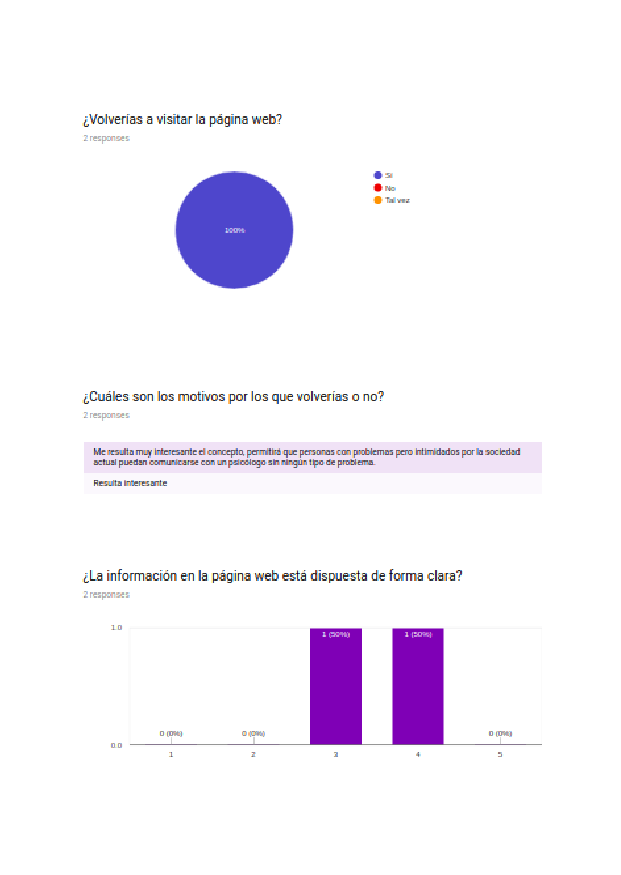
\includepdf[pages=-]{capitulos/test_usabilidad/test_usab_pac.pdf}


\newpage


\subsubsection{Test de usabilidad de los psicólogos}
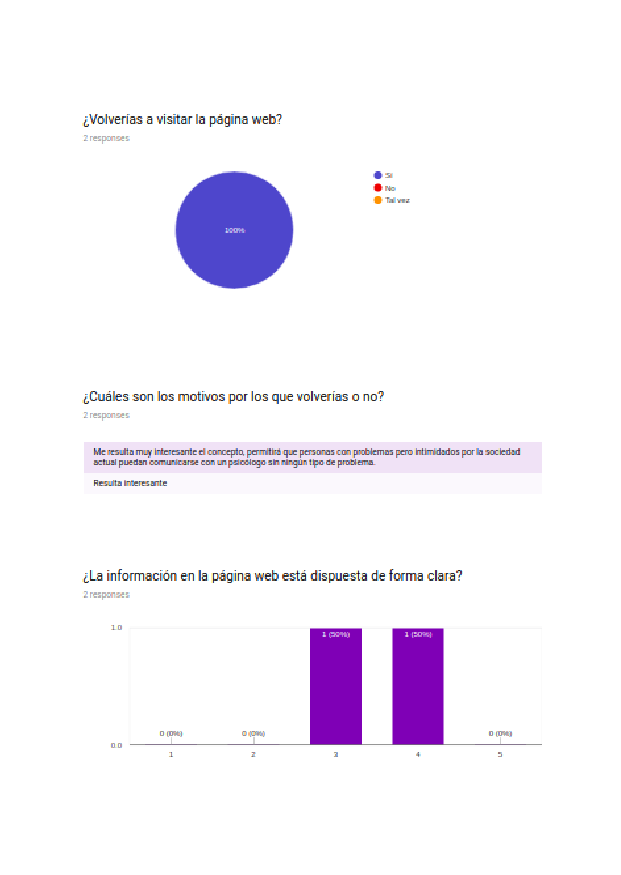
\includepdf[pages=-]{capitulos/test_usabilidad/test_usab_psic.pdf}


\newpage


\begin{table}[htpb]
\centering
\begin{tabularx}{\textwidth}{|l|X|X|}
\hline
\rowcolor[gray]{0.9}\textbf{Anexo PI-013} & \multicolumn{2}{l|}{\textbf{Prueba de accesibilidad}}                                                                                          \\ \hline
\textbf{Página}       & \textbf{Errores}                                                                           & \textbf{Solución}                                 \\ \hline
inicio.html           & El contraste entre el fondo y el elemento del contenido no es suficiente: Botón “Acceder”. & Se considerará la elección de un color diferente. \\ \hline
\end{tabularx}
\caption{Anexo PI-013}
%\label{my-label}
\end{table}


\begin{table}[htpb]
\centering
\begin{tabularx}{\textwidth}{|l|X|X|}
\hline
\rowcolor[gray]{0.9}\textbf{Anexo PI-013}    & \multicolumn{2}{l|}{\textbf{Prueba de accesibilidad}}                                                                                                                                                                                                                                             \\ \hline
\textbf{Página}          & \textbf{Errores}                                                                           & \textbf{Solución}                                                                                                                                                                                    \\ \hline
pacientesResultados.html & El contraste entre el fondo y el elemento del contenido no es suficiente: Botón “Filtrar”. & Se considerará la elección de un color diferente.                                                                                                                                                    \\ 
                         & Los atributos “id” de la página no son únicos.                                             & Se trata de los ids asociados a los containers de los psicólogos y que contienen los mismos atributos. Es el mismo elemento de contenido dispuesto de manera recursiva, por lo que no se modificará. \\ \hline
\end{tabularx}
\caption{Anexo PI-013}
%\label{my-label}
\end{table}


\begin{table}[htpb]
\centering
\begin{tabularx}{\textwidth}{|l|X|X|}
\hline
\rowcolor[gray]{0.9}\textbf{Anexo PI-013}      & \multicolumn{2}{l|}{\textbf{Prueba de accesibilidad}}                                                                                                                                                               \\ \hline
\textbf{Página}            & \textbf{Errores}                                                                                                                                                & \textbf{Solución}                                 \\ \hline
cuestionarioPacientes.html & El contraste entre el fondo y el elemento del contenido no es suficiente: Botón “Sí” activado o “No” activado. & Se considerará la elección de un color diferente.                                                                                                                                                    \\ \hline
\end{tabularx}
\caption{Anexo PI-013}
%\label{my-label}
\end{table}


\begin{table}[htpb]
\centering
\begin{tabularx}{\textwidth}{|l|X|X|}
\hline
\rowcolor[gray]{0.9}\textbf{Anexo PI-013}               & \multicolumn{2}{l|}{\textbf{Prueba de accesibilidad}}                                                                                                                                                                                                                                                                                                                                                                                                            \\ \hline
\textbf{Página}                     & \textbf{Errores}                                                                                                                                                                                                                                       & \textbf{Solución}                                                                                                                                                                                       \\ \hline
\multirow{2}{*}{pacientesMail.html} & El contraste entre el fondo y el elemento del contenido no es suficiente: Botones “Pendientes”, “Aceptadas” y “Rechazadas, etiqueta con el número de peticiones de cada tipo, etiqueta de estado de la petición “Pendiente de respuesta”. Texto del mensaje. & Se considerará la elección de un color diferente.                                                                                                                                                       \\ \cline{2-3} 
                                    & Los atributos “id” de la página no son únicos.                                                                                                                                                                                                         & Se trata de los ids asociados a cada uno de los mensajes enviados y al psicólogo remitente de los mismos. Es el mismo elemento de contenido dispuesto de manera recursiva, por lo que no se modificará. \\ \hline
\end{tabularx}
\caption{Anexo PI-013}
%\label{my-label}
\end{table}


\begin{table}[htpb]
\centering
\begin{tabularx}{\textwidth}{|l|X|X|}
\hline
\rowcolor[gray]{0.9}\textbf{Anexo PI-013}  & \multicolumn{2}{l|}{\textbf{Prueba de accesibilidad}}                                                                                                                                                                                                                                                                \\ \hline
\textbf{Página}        & \textbf{Errores}                                                                                                                                                               & \textbf{Solución}                                                                                                                   \\ \hline
registroPacientes.html & El contraste entre el fondo y el elemento del contenido no es suficiente: Botón “Acceder”, enlace “Términos y condiciones de uso”, botón “Registrar” y enlace “Registro de psicólogos” & Se considerará la elección de un color diferente para los botones, mientras que los enlaces se mantendrán con su color por defecto. \\ \hline
\end{tabularx}
\caption{Anexo PI-013}
%\label{my-label}
\end{table}


\begin{table}[htpb]
\centering
\begin{tabularx}{\textwidth}{|l|X|X|}
\hline
\rowcolor[gray]{0.9}\textbf{Anexo PI-013}   & \multicolumn{2}{l|}{\textbf{Prueba de accesibilidad}}                                                                                                                            \\ \hline
\textbf{Página}         & \textbf{Errores}                                                                                                             & \textbf{Solución}                                 \\ \hline
registroPsicologos.html & El contraste entre el fondo y el elemento del contenido no es suficiente: Botón “Acceder”, título de cada paso y botón “Siguiente” & Se considerará la elección de un color diferente. \\ \hline
\end{tabularx}
\caption{Anexo PI-013}
%\label{my-label}
\end{table}


\begin{table}[htpb]
\centering
\begin{tabularx}{\textwidth}{|l|X|X|}
\hline
\rowcolor[gray]{0.9}\textbf{Anexo PI-013} & \multicolumn{2}{l|}{\textbf{Prueba de accesibilidad}}                                                                                                                                                                                                                                                                                                                                     \\ \hline
\textbf{Página}       & \textbf{Errores}                                                                                                                                                 & \textbf{Solución}                                                                                                                                                                                                      \\ \hline
\multirow{2}{*}{psicologosMail.html}   & El contraste entre el fondo y el elemento del contenido no es suficiente: Mismos botones y etiquetas que en PacientesMail.html, botón “Aceptar” y título “Diagnóstico” & Se considerará la elección de un color diferente.                                                                                                                                                                      \\ \cline{2-3} 
                      & Los atributos “id” de la página no son únicos.                                                                                                                   & Se trata de los ids asociados a cada uno de los mensajes enviados y al diagnóstico del paciente remitente de los mismos. Es el mismo elemento de contenido dispuesto de manera recursiva, por lo que no se modificará. \\ \hline
\end{tabularx}
\caption{Anexo PI-013}
%\label{my-label}
\end{table}


\begin{table}[htpb]
\centering
\begin{tabularx}{\textwidth}{|l|X|X|}
\hline
\rowcolor[gray]{0.9}\textbf{Anexo PI-013} & \multicolumn{2}{l|}{\textbf{Prueba de accesibilidad}}                                                                                                                                                                                                                                                                                 \\ \hline
\textbf{Página}       & \textbf{Errores}                                                                                                                                                         & \textbf{Solución}                                                                                                                                          \\ \hline
\multirow{2}{*}{perfilPsicologo.html}  & El contraste entre el fondo y el elemento del contenido no es suficiente: Títulos “Formación”, “Experiencia” y “Especialidad” y; fecha y botón “Responder” de cada comentario & Se considerará la elección de un color diferente.                                                                                                          \\ \cline{2-3} 
                      & Los atributos “id” de la página no son únicos.                                                                                                                           & Se trata de los ids asociados a cada uno de los comentarios. Es el mismo elemento de contenido dispuesto de manera recursiva, por lo que no se modificará. \\ \hline
\end{tabularx}
\caption{Anexo PI-013}
%\label{my-label}
\end{table}


\section{Pruebas de navegación}

\subsection{Incrementos 1 y 2}
Anexos PN-001 y PN-002.

\begin{table}[htpb]
\centering
\begin{tabularx}{\textwidth}{|X|X|}
\hline
\rowcolor[gray]{0.9}\textbf{PN-001: USN-003, USN-004, USN-008, USN-009}                                                                                                         & \textbf{Evaluación}                                 \\ \hline
¿La USN se logra en su totalidad sin error?                                                                                                                & Sí                                                  \\ \hline
¿Todo nodo de navegación (definido por una USN) se alcanza dentro del contexto de las rutas de navegación definidas por la USN?                            & Sí                                                  \\ \hline
¿Existe un mecanismo (distinto a la flecha ``retroceso'' del navegador) para regresar al nodo de navegación anterior y al comienzo de la ruta de navegación? & No aplica - La profundidad de la navegación es de 1 \\ \hline
¿Los mecanismos de navegación dentro de un gran nodo de navegación (es decir, una página web grande) funcionan de manera adecuada?                         & Sí                                                  \\ \hline
Si una función debe ejecutarse en un nodo y el usuario elige no proporcionar entrada, ¿el resto de la USN puede completarse?                               & Sí                                                  \\ \hline
Si una función debe ejecutarse en un nodo y ocurre un error en el procesamiento de la función, ¿la USN puede completarse?                                  & Sí                                                  \\ \hline
¿Los nombres de nodo son significativos para los usuarios finales?                                                                                         & Sí                                                  \\ \hline
¿El usuario entiende su ubicación dentro de la arquitectura de contenido conforme se ejecuta la USN?                                                       & Sí                                                  \\ \hline
\end{tabularx}
\caption{Anexo PN-001}
%\label{my-label}
\end{table}


\begin{table}[htpb]
\centering
\begin{tabularx}{\textwidth}{|X|X|}
\hline
\rowcolor[gray]{0.9}\textbf{PN-002: USN-001, USN-002, USN-006, USN-010}                                                                                                         & \textbf{Evaluación}                              \\ \hline
¿La USN se logra en su totalidad sin error?                                                                                                                & Sí                                               \\ \hline
¿Todo nodo de navegación (definido por una USN) se alcanza dentro del contexto de las rutas de navegación definidas por la USN?                            & Sí                                               \\ \hline
¿Existe un mecanismo (distinto a la flecha ``retroceso'' del navegador) para regresar al nodo de navegación anterior y al comienzo de la ruta de navegación? & No aplica - La profundidad de navegación es de 1 \\ \hline
¿Los mecanismos de navegación dentro de un gran nodo de navegación (es decir, una página web grande) funcionan de manera adecuada?                         & Sí                                               \\ \hline
Si una función debe ejecutarse en un nodo y el usuario elige no proporcionar entrada, ¿el resto de la USN puede completarse?                               & Sí                                               \\ \hline
Si una función debe ejecutarse en un nodo y ocurre un error en el procesamiento de la función, ¿la USN puede completarse?                                  & Sí                                               \\ \hline
¿Los nombres de nodo son significativos para los usuarios finales?                                                                                         & Sí                                               \\ \hline
¿El usuario entiende su ubicación dentro de la arquitectura de contenido conforme se ejecuta la USN?                                                       & Sí                                               \\ \hline
\end{tabularx}
\caption{Anexo PN-002}
%\label{my-label}
\end{table}


\subsection{Incremento 3}

Anexo de la PN-006.

\begin{table}[htpb]
\centering
\begin{tabularx}{\textwidth}{|X|X|}
\hline
\rowcolor[gray]{0.9}\textbf{PN-004: USN-005, USN-007, USN-011, USN-012}                                                                                                         & \textbf{Evaluación}                                 \\ \hline
¿La USN se logra en su totalidad sin error?                                                                                                                & Sí                                                  \\ \hline
¿Todo nodo de navegación (definido por una USN) se alcanza dentro del contexto de las rutas de navegación definidas por la USN?                            & Sí                                                  \\ \hline
¿Existe un mecanismo (distinto a la flecha ``retroceso'' del navegador) para regresar al nodo de navegación anterior y al comienzo de la ruta de navegación? & No aplica -- La profundidad de la navegación es de 1 \\ \hline
¿Los mecanismos de navegación dentro de un gran nodo de navegación (es decir, una página web grande) funcionan de manera adecuada?                         & Sí                                                  \\ \hline
Si una función debe ejecutarse en un nodo y el usuario elige no proporcionar entrada, ¿el resto de la USN puede completarse?                               & Sí                                                  \\ \hline
Si una función debe ejecutarse en un nodo y ocurre un error en el procesamiento de la función, ¿la USN puede completarse?                                  & Sí                                                  \\ \hline
¿Los nombres de nodo son significativos para los usuarios finales?                                                                                         & Sí                                                  \\ \hline
¿El usuario entiende su ubicación dentro de la arquitectura de contenido conforme se ejecuta la USN?                                                       & Sí                                                  \\ \hline
\end{tabularx}
\caption{Anexo PN-004}
%\label{my-label}
\end{table}